\documentclass[12pt]{article} 
\usepackage{epsfig} 
\usepackage{graphicx} 
\begin{document}
\section{Trigger Scintillator Counters}
\subsection{Overview}

The trigger on each spectrometer includes two planes of trigger scintillators S1 and S2.
In addition, the HA detector stack includes optional third plane, S3. The mounting schemes
of these planes are different. S1 clamped to the Detector Frame through additional 
aluminum channel. S2 assembled on the sub frame, which can be slide on the rails into Detector Frame.
S3 has strong heavy sub frame, which can be mounted on the top of HA Detector Frame.  
The S1 and S2 planes each consists of six paddles. S1 paddle has active area 29.5 cm by 35.5 cm.
S2 paddle has active area 54.0 cm by 37.0 cm. The counters made of 5 mm thick BICRON 
408 plastic scintillator. Each paddle viewed with two 2" photo multiplier tubes Burle 8575. 
Light guides made of six lucid strips with long cylindrical spool at the end. There is 
an inlet for optical fiber mounted on the side of the cylindrical part of light guide.
S1 paddles are installed at small angle to the average S1 plane. S1 paddles have overlap by 10 mm. 
Paddles are supported from PMT housings ( see figure~\ref{S1_mounting} ). 
S2 paddles have only 5 mm overlap. Paddles supported right 
outside the active area to minimize deflection of the plastic scintillator and value of 
torque applied to the mounting of the PMT housing.

\begin{figure}
\begin{center}
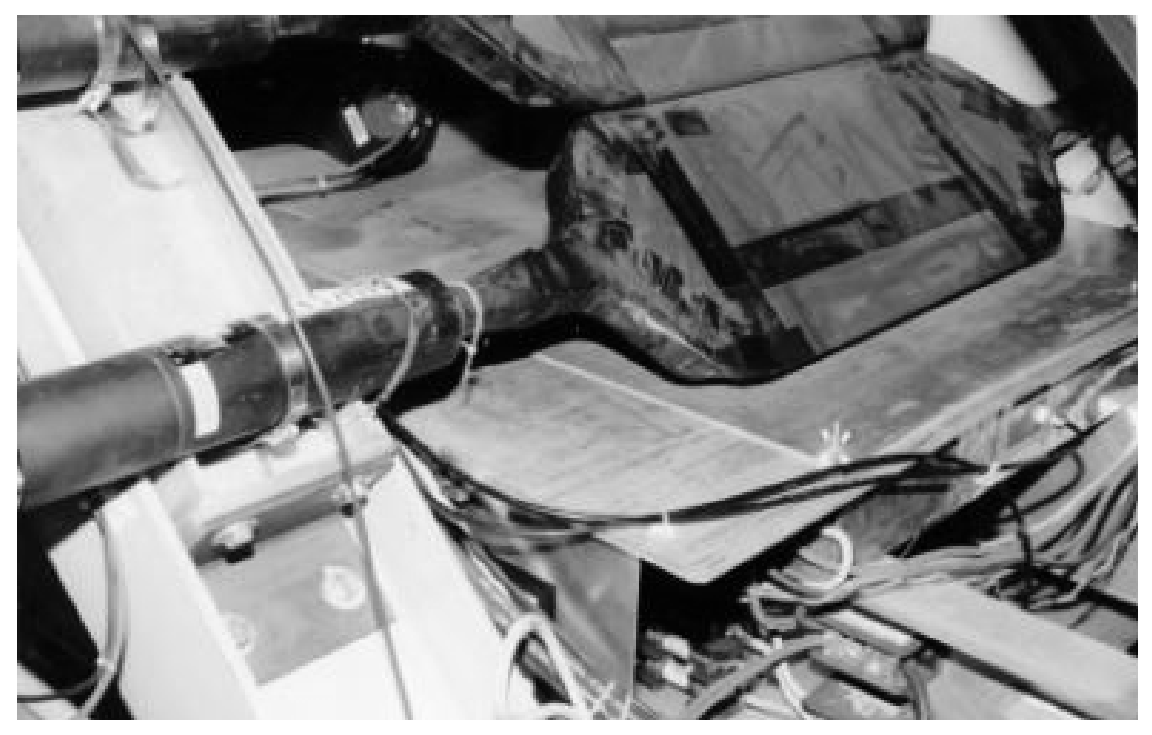
\includegraphics[width=15cm,clip]{scint_fig5.eps}
{\linespread{1.}
\caption[S1 mounting scheme]{S1 mounting}
\label{S1_mounting}}
\end{center}
\end{figure}

\subsection{Operation}
\subsubsection{Amplitude and time resolution}

There are 400-500 photons per event which reach the photo cathode of each side of the counters.
For fresh PMT it leads to 80-100 photo electrons. On HRS we are using discriminators with 
threshold 45 mV so PMT gain should be $\sim 3*10^6$. For fresh PMT this gain correspondent to 
HV in the range of 1800-2000 V. 
Amplitude variation from one end of active area to another is about 30\%. 
Based on PMT pulse rise time ( $ \sim 2.8 $ ns ) and photo electron statistics estimated time resolution 
is about 0.20 ns. On cosmic rays the time resolution ( sigma ) was observed about $\sim 0.30$ ns.  
Time propagation of the light inside detector varies by 10 ns across the active area. This effect 
is taken into account by using track position information.

\subsubsection{HV power supply} 
LeCroy HV 1460 used to supply HV power for trigger counters. It can be controlled from 
VT100 terminal connected through terminal server or through EPICS system based on computer HAC. 
Current HV settings for trigger counters should be found from print of EPICS control in the 
last experimental logbook.   
The example on figure~\ref{HVwindowEPICS} and
figure~\ref{HVcardEPICS} below included to present text for guidance only as help to identify 
the correct windows of the EPICS system. The settings used on these plots may be not correct.

\begin{figure}
\begin{center}
\includegraphics[width=15cm,height=16cm,clip]{scint_hv.eps}
{\linespread{1.}
\caption[HV control window]{EPICS control for detector HV system}
\label{HVwindowEPICS}}
\end{center}
\end{figure}

\begin{figure}
\begin{center}
\includegraphics[width=12cm,height=16cm,clip]{scint_hvcard.eps}
{\linespread{1.}
\caption[HV control for one card]{EPICS control window for one card}
\label{HVcardEPICS}}
\end{center}
\end{figure}

\begin{figure}
\begin{center}
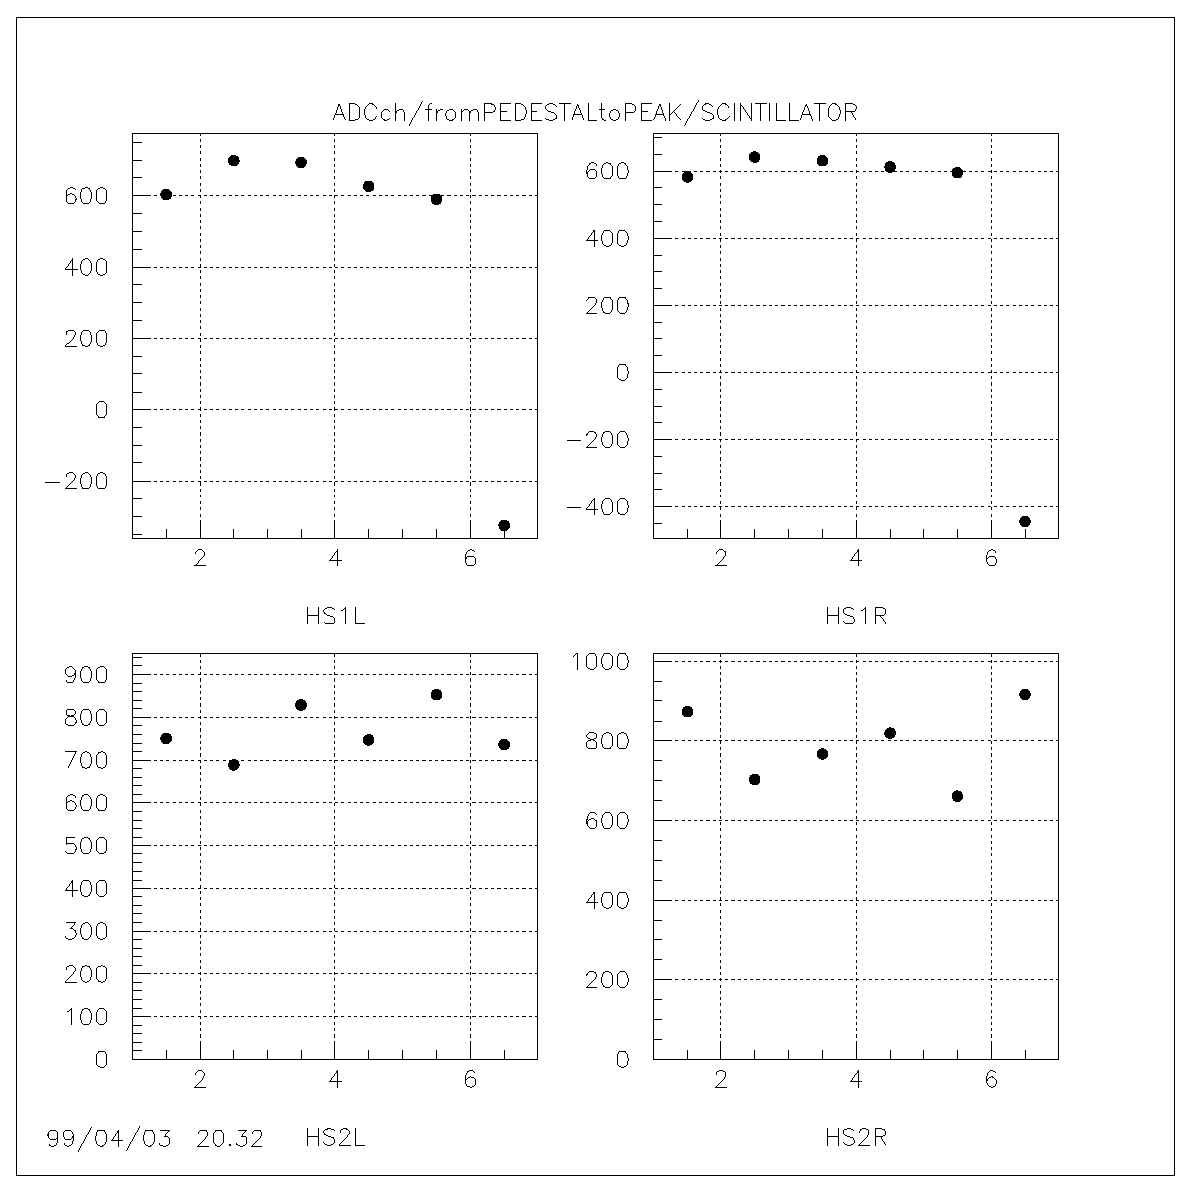
\includegraphics[angle=0,width=12cm,height=16cm]{scint_fig7.eps}
{\linespread{1.}
\caption[Kazu results]{Average amplitudes of PMT signals for HA trigger counters}
\label{kazu_results}}
\end{center}
\end{figure}

\subsubsection{PMT rate and gain monitoring}
There are two ways to monitor PMT and detector performance. The first one is based on scaler 
display program {\it xscaler}, which provides information about PMT counting rates and 
coincidence counting rates.
The large variation of the rates between paddles is an indication of possible problem.
The second way uses the analysis code ESPACE and kumac files developed by K. Takahashi 
(``kazu'' files). The analysis provides the amplitude spectra for events with good track in VDC.
It makes the histograms of the amplitudes and find average amplitudes for each PMT. For high efficiency
of the trigger it is important to keep average amplitude above 600 channels. The example of
analysis result shown on figure~\ref{kazu_results}.

\subsubsection{PMT replacement}
The air around detectors has sometimes large fraction of He. This gas diffuses quickly 
into some of PMT. As result of poor vacuum inside of PMT there is after-pulse effect
which caused by ions produced near anode in electron avalanche. Ions are bombarding the photo 
cathode. The photo cathode evaporation is a reason of slow diminishing of the quanta efficiency 
of the PMT ( up to $\sim 10-20 \%$ per month in case of high rate operation ). 
PMT should be replaced in the following cases:
HV exceed 2500 V and average amplitude is below 600 channels; counting rate is much higher then 
for other PMT, which indicate large probability of after pulses; efficiency is less then $95\%$.
The procedure of replacement for one PMT takes about $\sim$ 15-20 minutes.

\subsection{ 2" PMT Bases for S1 and S2 Trigger Counters}

\begin{figure}
\begin{center}
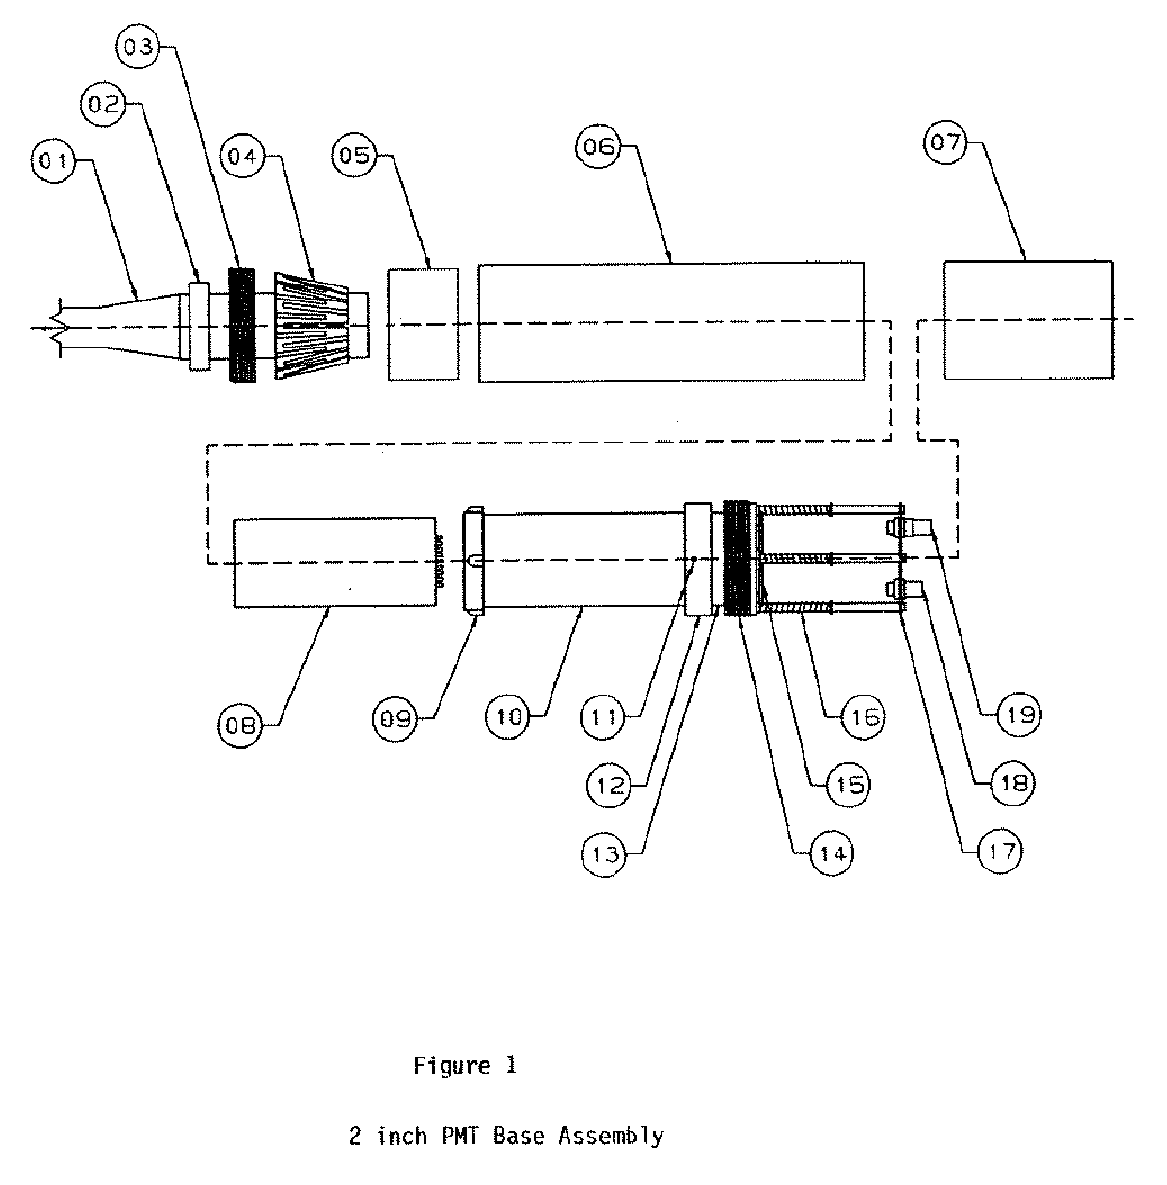
\includegraphics[width=15cm,clip]{scint_fig1.eps}
{\linespread{1.}
\caption[The 2" PMT base assembly used in S1 and S2 trigger scintillators]{2'' PMT base assembly}
\label{2''_PMT_base_assembly}}
\end{center}
\end{figure}

A schematic diagram of the 2" PMT Base assembly is shown in figure~\ref{2''_PMT_base_assembly}. 
The Base assembly consists of three main components. 
Front Tubular Housing (06), which encloses the PMT, part of the scintillator 
counter's light guide (01), and the mu-metal shield (10). The actual base with 
the socket and dynode chain is a separate part, actually an assembly of parts 
(09-19). The Rear Tubular Housing (07) completes the assembly and encloses the 
dynode chain and wiring. The three main sections join at the coupling nut (14), 
which threads partly inside the front tubular housing, while the rear tubular 
housing threads on the remaining part.

The PMT and the electronic amplification components mounted on a PC board 
(15) are enclosed in an aluminum Faraday cage, which assures rigidity and 
protection from stray RF fields. The mu-metal shield is at cathode potential to 
minimize the dark current due to capacitance discharge in the photo cathode 
glass window.

\begin{figure}
\begin{center}
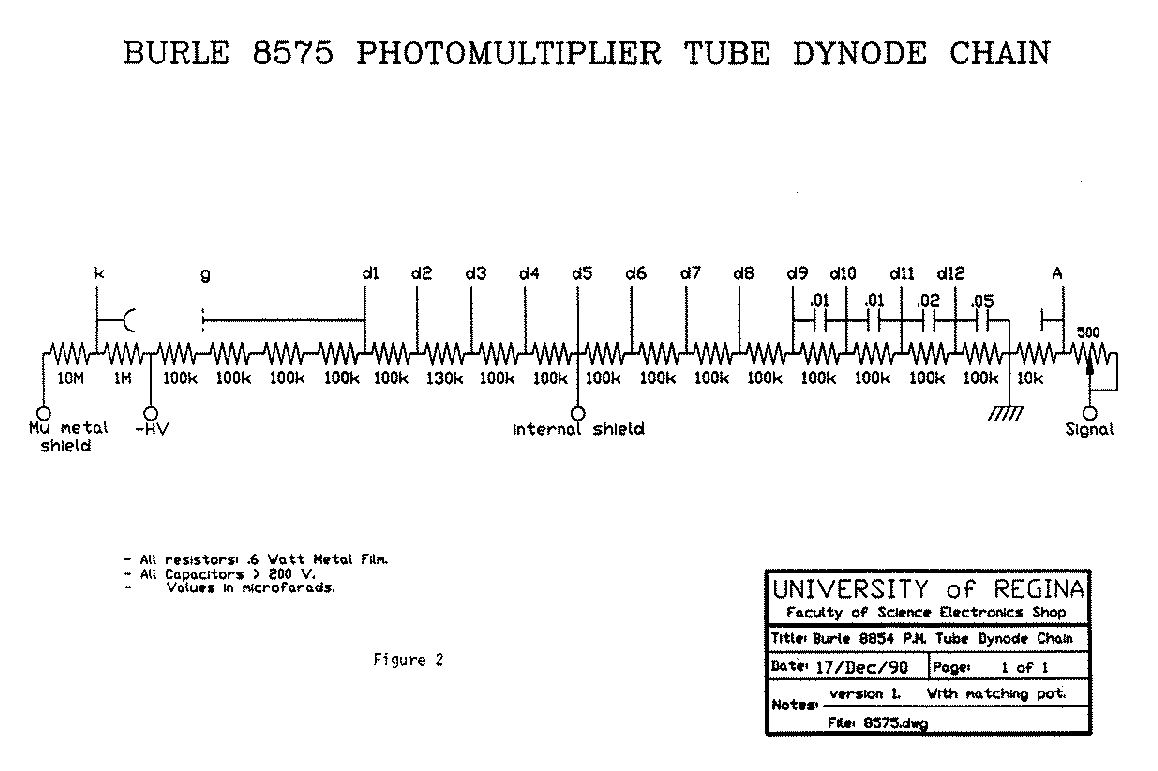
\includegraphics[width=15cm,clip]{scint_fig2.eps}
{\linespread{1.}
\caption[The 2" PMT base used in S1 and S2 trigger scintillators]{2'' PMT dynode chain}
\label{2''_PMT_dynode_chain}}
\end{center}
\end{figure}

\subsubsection{Handling Considerations}
\paragraph{Assembly Instructions}

   Unscrew the rear tubular housing from the coupling nut and then unscrew the
front tubular housing from the coupling nut, as well.  Remove the mu-metal
shield (10) from the retainer ring (12) by loosening the nylon locking set screw
(11). After insertion of the PMT in the socket, install the mu-metal shield and
make sure it sits squarely in the bottom of the socket base (13). 

WARNING: The mu-metal shield should NEVER be assembled in the base without the 
plastic insulator ring (09). Electrical shock may result if someone touches the 
outside housings under such a condition. The plastic insulator ring also serves 
as a mechanical alignment aid to keep the mu-metal shield centered within the 
front tubular housing.

Tighten the nylon locking set screw but don't over do it and strip the nylon
threads in the process. The mu-metal shield has a solid friction fit in the
copper ring inside the retainer ring to make good electrical contact. 

Screw the base assembly, with the PMT and mu-metal shield attached, back into
the front tubular housing, up to the half way point of the threads in the
coupling nut. The PMT socket and dynode chain assembly (15) is spring loaded
(16) so one can see how much compression the light guide will induce on this
assembly, thus assuring a good contact with the PMT without the risk of damage
to the latter. Insert the collet nut (03) and the inner collet (04) onto the
light guide as shown in figure~\ref{2''_PMT_base_assembly}. Position the outer collet inside the entrance
to the front tubular housing and check that it matches the direction of the
cone to that of the outer collet. Smear a thin layer of optical grease on the
light guide and insert the latter into the inner collet until it makes contact
with the PMT. This can be verified by observing the movement of the socket
against the, now slightly compressed, springs. Insert the outer collet into the
inner one and screw the collet nut making sure the springs remain slightly
compressed in the process. Use the special tool to tighten the collet nut until
the light guide cannot be moved in or out. 

Replace the rear tubular housing by screwing it all the way into the coupling 
nut. Insert the foam plastic light stop (02) between the collet nut and the 
light guide. The mechanical assembly is now complete. 


\paragraph{The Electronic Amplification Chain}

   The arrangement of the resistor dynode chain is shown in figure~\ref{2''_PMT_dynode_chain}. The 
cathode is connected to the mu-metal shield through a 10 MOhm resistor, in
addition to the 1 MOhm resistor between the cathode and the negative HV. The
dynode chain incorporates an adjustable potentiometer (0-500 Ohms) to allow a
match between the PMT and the external load, in order to eliminate after-pulse
ringing.  This potentiometer should be adjusted at first to 250 Ohm and then
make fine adjustments as needed by observing the anode pulses on the
oscilloscope for critical matching. It is not advised to do the adjustments
with HV on. Instead, the process should be done with HV off, remove the rear
tubular housing, adjust the potentiometer, replace the rear housing, and then
HV on again. Iterate until the matching is accomplished. In addition to the
obvious safety concerns, one does not want to remove the light sealing rear
housing from an active PMT and induce a large light leak which could destroy
the PMT. 

   Both 2" and 5" bases have been extensively tested under beam conditions. 
They have several safety related features but these cannot protect anyone who 
is bent on violating operating procedures and common sense. They allow the 
removal of the PMT/Base assembly, for repairs of the electronics or replacement 
of a PMT, without decoupling the housing and collets from the light guide. 
Thus, replacement of PMTs can be done in minutes without the need to remove the 
scintillator counters from their subframes.

\begin{figure}
\begin{center}
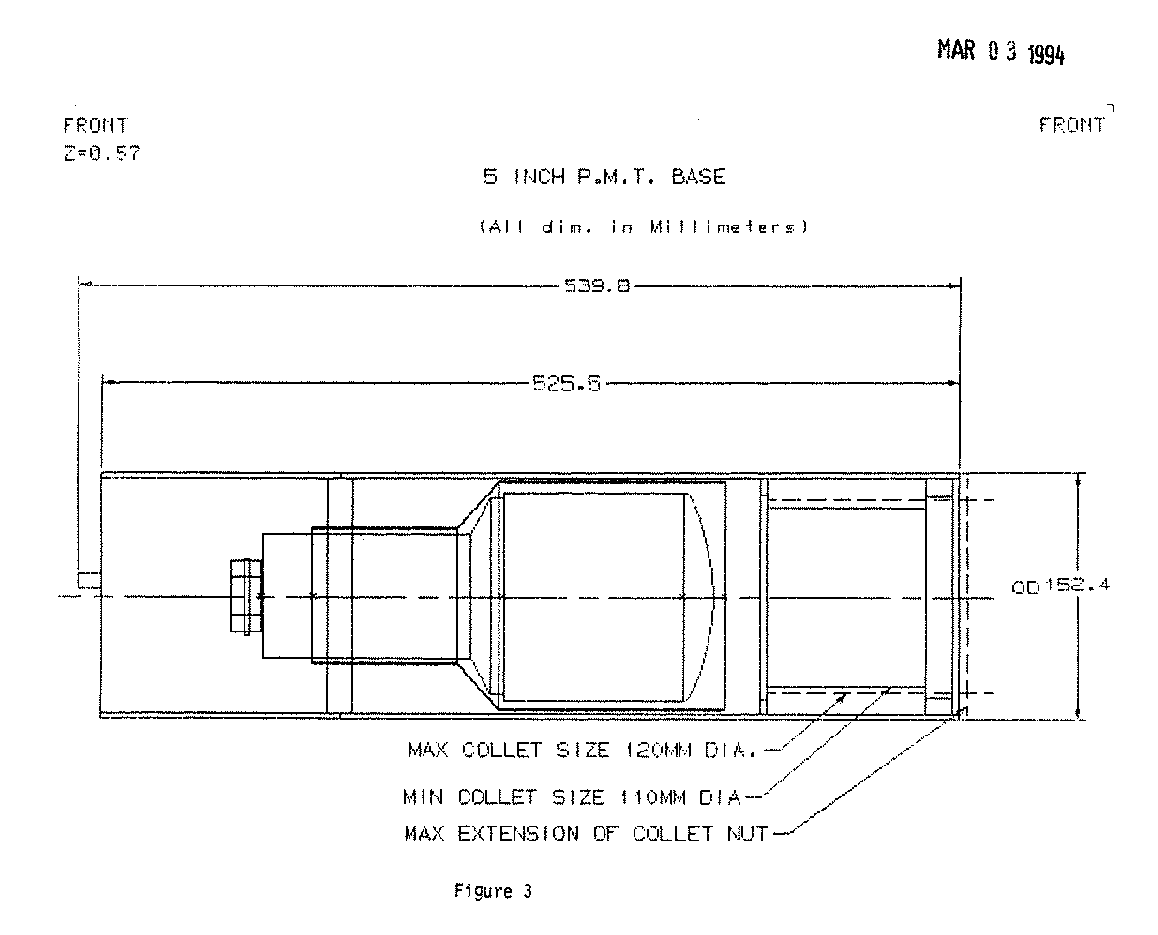
\includegraphics[width=15cm,clip]{scint_fig3.eps}
{\linespread{1.}
\caption[The S3 trigger scintillators]{5'' PMT assembly}
\label{5''_PMT_assembly}}
\end{center}
\end{figure}

\subsection{ 5" PMT Bases for S3 Counters}

   The general layout of the 5" PMT Base assembly is similar to that of the 2" PMT
described above. It consists of a front tubular housing and a rear tubular
housing, both made out of aluminum. They join at a coupling nut, as shown in
the schematic diagram of figure~\ref{5''_PMT_assembly}. The actual base where the PMT, $\mu$-metal
shield, and the electronic dynode amplification chain are located, is
different. The corresponding middle section, incorporating the above
components, is made out of a molded structure used in both the 5" bases and
the aerogel Cherenkov counters. The PMT socket is molded integral to the
section and it is also spring loaded. The collets are different, due to the
size of the light guide, but the method of assembly is very similar to that of
the 2" PMT assemble. 

\begin{figure}
\begin{center}
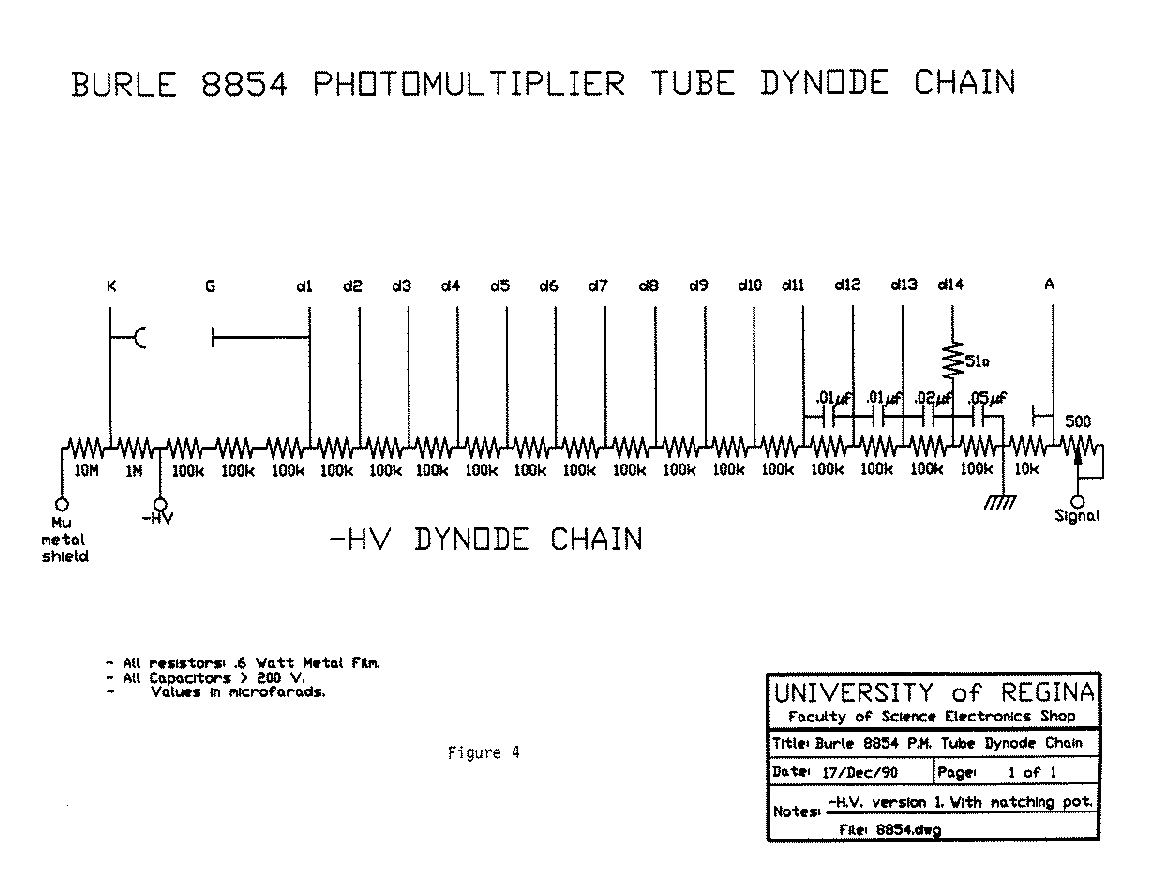
\includegraphics[width=15cm,clip]{scint_fig4.eps}
{\linespread{1.}
\caption[The 5" PMT base used in S3  trigger scintillators]{5'' PMT dynode chain}
\label{S3_PMT_dynode_chain}}
\end{center}
\end{figure}

\paragraph{Assembly Instructions}

   The collet assembly consists of several expanding rings, one set of solid
tapered and the other a spring collet. They are placed on top of each other,
alternating between the two kinds, with a spring collet on the top facing the
scintillator and the collet nut. As the collet nut is screwed in it presses
against the assembly and the spring collets slide inward against the tapered
solid ones, thus clamping against the light guide. Care should be taken, when
placing these two different kind of collets inside each other, so as not to
align the gaps in the plastic and create light leaks. The collets are not
continuous rings, otherwise they would not be compressible, and the gaps can
allow light all the way into the PMT if they are aligned. 

The collet nut is placed first around the light guide and the successive layers 
of the molded collets are then placed around the light guide; one should make 
sure that enough free length of exposed light guide remains to enter the 
housing to slightly compress the PMT and base assembly, as in the case of the 
2" base. Once the slight compression of the spring loaded PMT-socket assembly 
is verified, the set of collet rings is moved to enter the housing and rest 
firmly against the snap/stop ring inside the front tubular housing. Then the 
collet ring is screwed in using the special tool until the light guide is 
firmly bedded in the housing and cannot be moved in or out. The remaining 
procedure is the same as that of the 2" base.

Due to the two diameter shape of the 5" PMT and its mu-metal shield, insertion  
of the PMT pins into the socket is a blind operation. It has to be done by feel 
and experience; the pins can only go in a specific PMT-socket geometry and it 
needs experience to learn when the correct alignment has been achieved. Let 
someone who has experience do it, bending of the socket pins at the base of the 
PMT result in destroyed PMTs, and they are expensive.

WARNING: The plastic insulator sleeve inside the front tubular aluminum 
housing should be in place BEFORE the mu-metal shield/PMT assembly is inserted. 
Failure to assure the proper location of the insulating plastic sleeve may 
result in electrical shock.
 
\paragraph{The Electronic Amplification Chain}


The dynode amplification chain is mounted on a PC board, as is the case of the 
2" base. A schematic diagram of the resistor chain is shown in 
figure~\ref{S3_PMT_dynode_chain}. As in 
the case of the 2" base, it incorporates an adjustable potentiometer (0-500 
Ohm) and the nominal critical matching value is 90 Ohm. It has, in addition, a 
51 Ohm resistor in series with the 14th dynode, to further improve the shape of 
the anode pulse. A safe -HV to start with is -1,800 V; it provides the best 
timing resolution with adequate pulse height for electrons during in beam 
testing.

   Both 2" and 5" bases have been extensively tested under beam conditions. 
They have several safety related features but these cannot protect anyone who 
is bent on violating operating procedures and common sense. They allow the 
removal of the PMT/Base assembly, for repairs of the electronics or replacement 
of a PMT, without decoupling the housing and collets from the light guide. 
Thus, replacement of PMTs can be done in minutes without the need to remove the 
scintillator counters from their subframes.



\subsection{Safety Assessment}

WARNING: The bases are high voltage devices and should only be handled by 
competent people who can exercise common sense.

   The maximum voltage for both the PMTs and dynode chain is 3,000 V. In actual 
use, however, there should be no need to exceed of 2,500 V at operating 
parameters, since both PMTs and dynode chain have high gain. Nevertheless, the 
bases are high voltage devices and care should be exercised during handling and 
set up. The external aluminum parts, the front and rear housing, and the back 
plate (17), are all grounded via the ground of the BNC (18) and SHV (19) 
connectors. Since the back plate is connected to the coupling nut via the three 
steel posts, the front plate is also grounded via the coupling nut and the back 
plate. Common sense, however, dictates that the bases are not to be handled     
while under high voltage, even when multiple grounding connections are provided.

The mu-metal shield is also under high voltage, since it is connected to the 
cathode. Electrical isolation between the mu-metal shield and the front 
tubular housing is assured by the high dielectric retainer ring (12) and the 
plastic insulator (09) at the free end of the mu-metal shield. The air gap 
between the mu-metal shield and the front tubular housing is 6 mm, thus the 
breakdown value (18,000 V) far exceeds the maximum 3,000 V of the PMT.

In the event that the mu-metal shield is inserted without the plastic insulator 
ring, or some oaf decides to operate the base without the outside housings, the 
11 MOhm resistors between the -HV and the mu-metal shield will restrict the 
current flow through the mu-metal shield (and the oaf's hands) to less than 0.2 
mA with -2,100 V on the base. 

\subsection{Responsible Personnel} 
The following individuals are authorized to work on trigger scintillator counters. 
\begin{itemize}
\item[~]Segal, Jack - x7242 
\item[~]Wojtsekhowski, Bogdan - x7191 
\end{itemize} 

\end{document}













